% Template for PLoS
% Version 1.0 January 2009
%
% To compile to pdf, run:
% latex plos.template
% bibtex plos.template
% latex plos.template
% latex plos.template
% dvipdf plos.template

\documentclass[10pt]{article}
\usepackage{amsmath}
\usepackage{amssymb}
\usepackage{graphicx}
\usepackage{color} % for revision purposes only, may be not present in the final file
% cite package, to clean up citations in the main text. Do not remove.
\usepackage{cite}
\usepackage{color}
\usepackage{indentfirst} %% LM: in order to indent the first paragraph of each section
\usepackage{url} %% LM: in order to include nice urls
\usepackage{booktabs} %% LM: nice tables...
\usepackage{subfigure} % LM: panels
\usepackage{xr} % automatic cross-referencing
\externaldocument{Text_S2}
% Use doublespacing - comment out for single spacing
%\usepackage{setspace}
%\doublespacing

\topmargin 0.0cm
\oddsidemargin 0.5cm
\evensidemargin 0.5cm
\textwidth 16cm
\textheight 21cm

\usepackage[labelfont=bf,labelsep=period,justification=raggedright]{caption}

\bibliographystyle{plos2009}% 

\makeatletter
\renewcommand{\@biblabel}[1]{\quad#1.}
\makeatother


% Leave date blank
\date{}

\pagestyle{myheadings}
%% ** EDIT HERE **


%% ** EDIT HERE **
%% PLEASE INCLUDE ALL MACROS BELOW

%% END MACROS SECTION

\begin{document}

% Title must be 150 characters or less
\begin{flushleft}
{\Large
\textbf{Spatiotemporal Dynamics of Foot-and-Mouth Disease Virus in South America}
}
% Insert Author names, affiliations and corresponding author email.
\\
Luiz Max Carvalho$^{1,2\ast}$,
Guy Baele$^{3}$,
Nuno Rodrigues Faria$^{3,4}$,
Andres M.~Perez$^{5}$,
Marc A.~Suchard$^{6,7}$
Philippe Lemey$^{3}$,
Waldemir de Castro Silveira$^{1}$
\\
\bf{1} Pan American Center for Foot-and-Mouth Disease (PAHO/WHO), Duque de Caxias, Rio de Janeiro, Brazil.
\\
\bf{2} Program for Scientific Computing (PROCC), Oswaldo Cruz Foundation, Rio de Janeiro, Rio de Janeiro, Brazil.
\\
\bf{3} Department of Microbiology and Immunology, Rega Institute -- KU Leuven, Leuven, Belgium.
\\
\bf{4} Department of Zoology, University of Oxford, Oxford, United Kingdon
\\
\bf{5} Department of Veterinary Population Medicine, University of Minnesota, St. Paul, United States of America.
\\
\bf{6} Departments of Biomathematics and Human Genetics, David Geffen School of Medicine at UCLA, University of California, Los Angeles,  United States of America.\\
\bf{7} Department of Biostatistics, UCLA Fielding School of Public Health, University of California, Los Angeles,  United States of America.
\\
$\ast$ E-mail: lmax.procc@gmail.com
\end{flushleft}

% Please keep the abstract between 250 and 300 words
\section*{Abstract}

Although foot-and-mouth disease virus (FMDV) occurrence has disminished over the years, the virus still circulates in certain areas of South America and the risk of re-emergence in previously free areas is a constant threat.
While the molecular epidemiology of FMDV in South America has been subject of several studies recently, an integrated quantitative approach to incorporate environmental and epidemiological data into the analyses is still lacking.
In this study, we apply state-of-art Bayesian phylogeography to the most comprehensive data sets of VP1 (1D) sequences from FMDV serotypes A and O collected in South America to date, to study the temporal and spatial variation of FMDV and test evolutionary hypotheses.
We found that South American FMDV serotypes A and O exhibit rate variation among lineages and evolve measurably, while being best fitted by different relaxed molecular clock models (A: log-normal; O: exponential).
The phylogeographic analysis showed significant viral flow between Venezuela, Colombia and Ecuador while Brazil, Uruguay and Argentina also formed a well-connected subnetwork.
Using data on livestock (cattle, sheep and pigs) trade and geographic distance also allowed us to assess the importance of each of these predictors in viral flow, showing geographic distance to be the best predictor of serotype A spatial spread while the trade of live cattle was the strongest predictor of serotype O spread on the continent.
%Finally, we offer a thorough appreciation of the sensitivity of our conclusions to biased location sampling.
% Maybe we should disclose some 'real' results here, like what was robust to sampling and what wasn't

Key-words: Phylogeography, foot-and-mouth disease virus, South America, animal trade, BEAST.

\section*{Author Summary} % 150--200 words
Foot-and-mouth diseases virus (FMDV) % MAS: I assume the Author Summary can be read independently of the Abstract or Main Text, so I redefined this acronym
is a rapidly evolving and highly infectious livestock pathogen.
In South America, although some molecular epidemiology studies are available, little is known about the virus phylodynamics.
In this paper we analyse all available VP1 sequences of FMDV serotypes A and O isolated in South America to unravel the spatial and temporal dynamics of the virus on the continent.
We show that both serotypes evolve measurably in South America and identify times to most comment recent ancestor of $\approx 70$ and $\approx 20$ years for serotypes A and O, respectively. 
However, spatially, serotype O presents a dispersal rate four times bigger than serotype A.
Additionally, we found that Brazil is a hub for serotype A spread but not for serotype O, while Colombia and Ecuador seem to be more important for serotype O dispersal on the continent.
We identified the trade of live cattle as the most important predictor of serotype O, while for serotype A geographic distances seem to best predict viral flow between South American countries.
Taken together, these results show that FMDV serotypes' different biology reflects in their different spatial dispersal patterns and reinforces the view that the trade of live cattle, specially across national %MAS: or did you mean "within"? LM: no, I meant across the borders, since our data concerns international trade.
borders (short range migration) is an important threat to control programmes.   

\section*{Introduction}

Foot-and-mouth disease virus (FMDV) is a rapidly evolving picornavirus and the causative agent of foot-and-mouth disease (FMD), the most important disease of domestic and wild cloven-hoofed animals~\cite{review}.
Three of the seven FMDV serotypes (A, O, and C) still circulate in certain areas of South America.
Identification of serotype C in recent decades was limited to one case in the Brazilian Amazons.
Serotype O has historically been the most prevalent serotype on the continent but, recently, it has been limited to the areas in the Andean region~\cite{andean}.
Serotype A has been being responsible for epidemics that are typically larger and more extended than those caused by other serotypes and that, in recent years, have been limited to the Southern cone of the continent~\cite{Perez2001,Malirat2012}.
%NRF emergences=outbreaks?
FMDV was probably introduced in South America in the late years of the 19th century, likely brought by European colonization~\cite{tully}. 
By the 1970's, FMD was widespread in South America, with occurrence of multiple subtypes in large-scale epidemics~\cite{Saraiva2003}.

% LM  Andres suggestion: either move the following paragraph above or get rid of it once and for all
% In 1987, as a consequence of the improving knowledge about disease ecosystems accumulated by the national programmes, began the Hemispheric Plan for the Eradication of FMD (PHEFA), elaborated and signed by South American countries as a continent-wide programme to strengthen national infra-structures, control animal trade and improve diagnostic and epidemiological investigation capabilities\cite{review_eradication}.
% Its main objective is to create and maintain FMD-free areas, thus improving the availability of meat, milk and other economically important livestock products~\cite{Saraiva2003,Saraiva2004,review_eradication,combining}. Considerable success has been achieved over the past years, with substantial reduction of FMD incidence in the late 1990's.
% Despite considerable success, with a significant reduction in the incidence of FMD in the late 1990s, episodic outbreaks in 2001, 2005 and 2011, in areas previously free represented a serious setback for PHEFA, compromising its goals by 2010~\cite{Saraiva2003,Saraiva2004}.

In South America, FMD control and eradication has traditionally been pursued using a combination of mass vaccination programs~\cite{vaccinationSA} along with control of movements from areas in which FMDV infection was suspected and passive and active surveillance programs that, with heterogeneous success, were intended to early detect the FMDV.
Phylogenetic analyses have already proved useful in the latter; particularly by recovering in real-time the transmission pathways from genetic data~\cite{cottam2007,cottam2008} and providing insight into the processes that drive re-emergence~\cite{combining}.
% In recent years, molecular epidemiology tools have been applied to understanding the (re-)emergence pattern of FMDV, allowing for inference on the origin and evolutionary history of emerging viruses~\cite{Perez2001,Malirat2007,andean,Malirat2011,Maradei2013}.
% These studies have played an important role in understanding the (re-)emergence pattern of FMDV, allowing for inference on the origin and evolutionary history of emerging viral strains~\cite{topotypes,Perez2001}.
% Together with vaccine matching and MAb profiling studies~\cite{Maradei2011}, phylogenetic analyses are a powerful 
% tool to evaluate control programmes and guide vaccine formulation~\cite{Maradei2011,Maradei2013}.

% The increased availability of geo-referenced time-stamped genetic data has fostered the development of new methods that integrate epidemiological and environmental data in order to reconstruct pathogen population dynamics and test evolutionary hypotheses~\cite{MEP,grenfell}. 
In recent years, molecular epidemiology tools have been applied to understand the (re-)emergence pattern of FMDV, allowing for inference of the origin and evolutionary history of emerging strains~\cite{Perez2001,Malirat2007,andean,Malirat2011,Maradei2013}.
However, as pointed out by Di Nardo, Knowles \&  Paton (2011)~\cite{combining}, a joint evaluation of epidemiological and environmental data is usually done outside of an unified quantitative framework, in a qualitative fashion.
In this context, Bayesian phylogeography offers a statistical framework to combine multiple sources of information in order to understand the spatio-temporal dynamics of FMDV and perform evolutionary hypothesis testing.
This framework has recently proven useful when investigating the patterns of FMDV spread and tracing the spatial origins of FMD epidemics~\cite{Carvalho2013,bulgaria,phymal,hall2013}.
% LM Andres comments : ''One may argue that in our early paper (3 in your reference list) we have already assessed time-space variation in relation to genetic variation in south America.
% There may also be other examples. I would use an alternative reasoning here. You are trying to assess the molecular epi of FMD at a continental level.
% This was done in the past (I believe Ingrid Bergmann and Viviana Malirat have published some work), but what never has been done is to reconstruct the history of evolution of the virus, and in relation to vaccination data, host-population dynamics, and time-space location. Make your case to demonstrate your originality.''
% TODO: whilst I disagree, I'd like to hear more from you boyz.

In this study, we analyse all publicly available VP1 (1D) sequences for FMDV serotypes A and O in South America (131 and 167 sequences, respectively).
Our data sets spanned over a long time-period (1955-2010 for serotype A and 1994-2010 for serotype O)  and cover nearly all South American countries affected by FMD.
We apply state-of-art Bayesian phylogeographic methods to investigate the evolutionary dynamics of serotypes A and O in South America, from both a spatial and temporal perspective.
The probabilistic framework used here allows for the incorporation of multiple sources of information to test hypotheses about viral dispersal, while naturally accommodating uncertainty~\cite{roots,towards}.

We use the Bayesian Evolutionary Analysis by Sampling Trees (BEAST) framework~\cite{beast2012} to infer time-structured phylogenies and a non-parametric demographic growth model~\cite{skyride} to reconstruct past population dynamics, to which we overlay  vaccination and serotype-specific notification data.
Moreover, we use data on livestock trade and geographical distances as predictors for viral spatial diffusion and use recently developed methods to more accurately estimate marginal likelihoods of competing spatial dynamics models involving each predictor.
% Finally, we offer an appreciation of the statistical hurdles that may be caused by biased geographic sampling, and propose ways to ameliorate their effects.
%TODO: decide whether or not this statement holds in the end; I think it's more of a referee thing, to preclude them from trashing our work

\section*{Results}

\subsection*{South American FMDV serotypes A and O exhibit rate variation among lineages and evolve measurably}

Analysis using jModelTest to select the evolutionary model yielded the general time reversible (GTR) model with a discretized gamma distributed across-site rate variation and a proportion of invariant sites (GTR+I+$\Gamma_{4}$) model as the best fit nucleotide substitution model for both FMDV data sets.
Next, we performed a computationally intensive model selection analysis to chose the best fitting demographic growth model and molecular clock model.
Our results indicate that the constant population assumption is rejected in favor of a model that allows fluctuations in demographic growth over time -- serotype A: log Bayes factor (BF) = $11$; serotype O: BF = $21$. % MAS: BF = 10 is certainly not decisive support LM: ``decisively'' is gone... ;0)

After, we found that both serotypes' rapid evolution better fits a relaxed than strict molecular clock model.
Particularly, the exponential relaxed molecular clock provided a better fit for serotype O data (log BF=$56$) while the log-normal relaxed molecular clock model provided a better fit to serotype A (log BF=$34$) 
% MAS: These numbers are very similar to those reported immediately above; I suspect an error. LM: somebody has an eagle eye... ;0) ; fixed
(see Table ~\ref{stab:treeclockselection} for details). 
The coefficient of variation for the log-normal relaxed molecular clock model had a posterior mean of $0.32$ (95\% highest posterior density [HPD] interval: $ 0.21$--$0.43$) 
% MAS: Or do you mean "highest posterior density interval" HPD? LM: that depends. Tracer gives the tangent set, my bad, its HPD...
indicating substantial rate heterogeneity among lineages in the phylogeny. 

A  `temporal signal' test~\cite{Faria2012} (see Methods) indicated significant temporal structure for both serotypes (A: log BF=$310$; O: log BF=$348$), showing that both FMDV data sets analysed here evolve measurably, a result also found for FMDV SAT 1 in East Africa~\cite{sangula}.

This finding is consistent with the view that FMDV presents clock-like evolution only when large periods of time are considered, with short periods being dominated by quasispecies dynamics~\cite{Muellner2011}.
Overall, these results show that sufficient temporal information is embedded in sequence data of both serotypes under investigation, which is central for the estimation of times of divergence and to reconstruct the population dynamics in natural time units~\cite{MEP}.
%TODO: Perhaps we should move this last paragraph to the Discussion?

\subsection*{Dating the divergence of FMDV isolates}

We performed a Bayesian analysis using BEAST to infer time-structured phylogenies for each FMDV serotype, assuming the corresponding best-fit combination of nucleotide substitution, demographic and molecular clock models.
The maximum clade credibility (MCC) tree estimated for serotype A (Figure~\ref{fig:trees}A) places the origin of the circulating strains in or around the early years of the 1920's decade.

Figure~\ref{fig:trees}A shows that sequences from the same country tend to cluster in small clades, although the inferred phylogenies for both serotypes also show considerable interspersing of lineages, indicating transborder FMDV spread.
For example, Argentinian serotype A sequences were grouped in two clades, that either comprised only Argentinian isolates or included sequences from Brazil and Uruguay (Figure~\ref{fig:trees}A).
Interestingly, the majority of the isolates from Venezuela and Colombia fall together within two distinct clades. 

Figure~\ref{fig:trees}B presents the estimated MCC tree for serotype O.
The same interspersing pattern can be noticed, with Ecuador and Colombia showing several interleaved clades.
The time to most recent common ancestor (tMRCA) for serotype O was estimated around 20 years, showing a more recent origin.
Here, a smaller clade of Colombian isolates are found interspersed within from Venezuelan isolates.
In addition, isolates from Ecuador are found interspersed with isolates from Colombia, suggesting that the intra-country dynamics of FMDV between these two countries is intrinsically linked.
Overall, the Bayesian phylogenies suggest that most FMDV flow within South America occurred between neighboring countries. 

Using the best fitting demographic and molecular clock model combination for each serotype, the evolutionary rate for serotype A was estimated at  $\approx 4 \times 10^{-3}$ substitutions/site/year.
In addition, the estimated evolutionary rate for serotype O was approximately 2.5 times faster than serotype A, i.e.~at $\approx 1 \times 10^{-2}$, consistent with previous studies~\cite{tully, Carvalho2013, Muellner2011}. 
% TODO: LM Andres claims that, for FMDV, we should only detect 'clockness' for data spanning over large periods. Whether this hold or not I don't know. The point is: we may include it into the discussion, but I don't think it jeopardizes any of the results of this section. Check related issue #32.
\begin{center}
 [Figure~\ref{fig:trees} about here]
\end{center}

\subsection*{Spatial Dynamics of FMDV in South America}

%To assess the spatial pattern of FMDV spread within South America, we performed Bayesian phylogeographic analysis, also using the models available in BEAST~\cite{roots}.
%We began by evaluating the spatial signal contained in our sequences using Bayesian tip-association tests~\cite{bats} to determine the amount of spatial signal in our reconstructed phylogenies.
%To gain insight into the amount of association for each location, we computed the maximum clade (MC) statistic.
The results of the spatial signal analysis using BaTS~\cite{bats} can be found in Table ~\ref{stab:BaTS} and show significant location-tip association for both serotypes.
As an overall summary, our data sets presented high degree of spatial signal, justifying richer phylogeographic analyses to study the transmission network of FMDV on the continent.

To gain insight into the spatio-temporal process of FMDV spread, we employed an asymmetric continuous-time Markov chain (CTMC) phylogeographic model~\cite{roots} available in BEAST~\cite{beast2012}, coupled with model averaging using Bayesian stochastic search variable selection (BSVSS) procedure (see Methods).
%BSSVS also naturally allows for the computation of Bayes factors, which are in turn used to assess the importance/significance of each migration path.
The results of the diffusion estimation are presented in Figure~\ref{fig:migration} and show that Brazil and Colombia were the most strongly connected regions (hubs) for both serotypes A and O.

The highest dispersal rates for serotype O were estimated for transitions between Colombia and Ecuador, Venezuela and Colombia and Uruguay and Argentina.
When we analysed support for various epidemiological linkage, the best supported (log BF$>9$) routes were between Peru and Brazil, Bolivia and Colombia, Uruguay and Argentina and Argentina and Peru.
The route between Uruguay and Peru showed smaller but strong support (log BF$>4$).

The highest dispersal rates for serotype A were obtained for transitions between Brazil and Uruguay, Ecuador and Venezuela and Bolivia and Venezuela.
When we looked at the epidemiological linkage, we found the transitions between Uruguay and Argentina, Argentina and Bolivia, Brazil and Argentina and Bolivia and Venezuela to have the highest support (log BF$>8$).

We notice that for serotype A mainly long-range migration routes were inferred for the period before 1945.
This result may be due to sparsity of information before 1970, that limits accurate inference about periods further back in time (see {\bf Discussion}). 
Also, there is a major expansion in spatial spread from 1945 to 1965, characterized by Brazil as a source of virus for the rest of the continent.
In the period 1965-1980, we note slower spread, mainly through short range routes.
The 1980-2008 window is characterized by FMDV serotype A flow into Peru and Paraguay and the increase of intra-country diversity (depicted by the radius of the displayed circles in Figure~\ref{fig:migration}).   

On the other hand, for serotype O expansion seems to have occurred by the middle of the 1990's.
Up to 1995, Colombia and Brazil appear to have acted as primary and secondary viral sources, respectively.
From 1995 to 2000, whilst Colombia acted as main source for the northern/Andean regions of the continent, spread in the Southern Cone seems to originate in Brazil.
The period 2000-2010 is characterized by a decrease in viral flow (almost no new edges added to the network) and the main feature is the increase in viral diversity within countries, specially Ecuador, Colombia and Brazil.

\begin{center}
 [Figure~\ref{fig:migration} about here]
\end{center}

To further explore the spatial behavior of FMDV, we infer
% MAS: Calling anything the "so-called XX" is a belittling statement in English: LM: I'm truly sorry, the 'so-called' thing was to stress the coloquial aspect of the name
``Markov jump'' (MJ) counts~\cite{Minin2008} that summarize the expected number of location state transitions along the  branches of the phylogeny and provide a quantitative measure of gene flow between countries, representing successful viral introductions from one region to another.
%For this analysis we also calculated BFs using BSSVS.
The results of the MJ analysis, along with the Bayes factors from BSSVS are presented in Figure~\ref{fig:mj&BFs} and show that supported migration routes differ for each serotype, with some overlapping routes connecting Venezuela, Colombia and Ecuador.
For serotype A, highest (log BF~$>800$) support was observed for viral flow between Venezuela and Colombia and between Argentina and Uruguay.
Transitions between Brazil and Bolivia and Peru and Ecuador also received good statistical support (log BF~$>10$).
For serotype O, overall support was lower in magnitude, but displaying similar routes.
Highest support was found for transition between Ecuador and Peru and Colombia and Ecuador (log BF~$>100$). Significant support was also observed for viral exchange between Venezuela and Colombia (log BF~$>20$). 

% Lots of short range routes are supported for both serotypes
%TODO: How to reconcile these results with the border vs non-border results below?

In order to study this pattern further, we compared the MJ counts between countries that share borders and those which do not.
The results show that for serotype A the posterior median transition count between neighbour countries was $0.02$ (95 \% BCI: $0.00$ -- $4.29$), while ``non-border'' transitions had a posterior median of $0.05$ (95 \% BCI: $0.00$ --  $3.39$).
For serotype O, similar results were observed, with $0.04$ ($0.00$ -- $1.99$) and $0.09$ ($0.00$ -- $1.25$) being observed for neighboring and non-neighboring countries, respectively.
Since the difference in medians is substantial but credible intervals widely overlap, we set up a Monte Carlo re-sampling experiment to calculate the probability that a randomly chosen ``border'' ($B$) transition is larger than a randomly chosen ``non-border'' (NB) one. For each data vector we obtained $100,000$ random draws and counted the number of times the above described event happened. From this experiment we found that the posterior $\mbox{Pr}(B>NB)$  to be $0.61$ for serotype A and $0.43$ for serotype O.

\begin{center}
 [Figure~\ref{fig:mj&BFs} about here]
\end{center}

% LM: methodological shit
%Using data from both serotypes jointly, we estimated marginal likelihoods for a model in which a single rate matrix was estimated (``shared'') and one in which two separate matrices were estimated (``separate''). 
%In the ``shared'' model we used trait (location) and sequence data  from both serotypes to make inference about one CTMC rate matrix, whilst in the ``separate'' model we allow both serotypes to have each one CTMC rate matrix, while using the combined data from both serotypes.
%Both models allow serotypes to have different spatial diffusion rates.
To investigate whether the two serotypes presented different spatial spread patterns, we plotted the dispersal rates estimated from independent runs for both serotypes and they do not seem to correlate (Figure~\ref{sfig:AvsO}).
%Moreover, from the separate and shared rate matrix analysis we found that rates inferred for serotype A are more strongly correlated with the rates estimated under a shared rate matrix, with Pearson's linear correlation coefficients $r_A=0.55$ and $r_O=0.18$, respectively.
%For this analysis, the correlation between serotype A and O rate matrix estimates was $0.07$.
%In contrast, the rate indicators in BSSVS for both serotypes were in better accordance ($r=0.54$).
%Again, we compared estimates using shared and separate models for the CMTC rate matrix, and found that indicators for serotype A had higher concordance to those in the shared model ($r_A=0.86$ and $r_O=0.77$).

%Using path sampling we obtained (log) marginal likelihoods of $-21478$ and $-21482$ for the shared and separate models respectively.
%Results from stepping stone sampling were $-21488$ and $-21492$ respectively.
%Bayes factors assessment of the statistical support for the two hypotheses (shared or separate rate matrices), indicated that a shared model should be preferred to a model with separate rate matrices for each serotype (BFs~$4$ and $10$ for PS and SS).

%Interestingly, shared and separate models yielded different most probable root locations for both serotypes.
%For serotype A the separate model yielded Argentina as the spatial origin ($Pr(\text{root})=0.52$, while the shared matrix model pointed Brazil as the root with probability of $0.57$.
%allowing two separate rate matrices Venezuela was pointed as most probable origin with probability $0.44$ and the model with a shared rate matrix pointed Colombia as root ($Pr(\text{root})=0.51$.

Regarding spatial signal extraction, analyses for serotypes  A and O yielded KL divergences of $1.93$ and $1.50$ respectively.
Overall, our analyses were slightly more efficient for serotype A in comparison with serotype O.

\subsection*{Identifying potential predictors of FMDV spread}

We used data on geographic distances and on trade of live cattle, pigs and sheep obtained from the detailed trade matrix available from the Food and Agriculture Organization (FAO), to elicit CMTC rate matrix priors (predictors).
By accurately calculating the marginal likelihood of a model involving each predictor, we gain insight into the importance of each variable on viral spread~\cite{Carvalho2013, Nelson2011}.
%We used data on geographic distances and on trade of live cattle, pigs and sheep.
%For each predictor, we performed MCMC runs using fixed root state frequencies for each country, with frequencies set to their observed values.
%Moreover we performed analyses where root state frequencies were estimated.
% LM : I'll restrict these remarks to Text S2 only
%The results of these experiments are presented in Text S2, Figure ~\ref{sfig:freqs}.
%We can observe that estimated frequencies considerably differ from their observed values.
%Moreover, the analyses with fixed frequencies yielded lower marginal likelihoods for the predictors (data not shown).
% All predictors were compared to a spatially uniform equal-rates prior using (log) Bayes factors.% LM: this is methods, I'll move it there and better explain it
%
Interestingly, the results of this analysis (Table~\ref{tab:preds}) show different best fitting predictors for each serotype.
For serotype A, distance and equal-rates outperform all the predictors tested, obtaining higher (log) marginal likelihoods.
For serotype O, the trade of live cattle as a predictor is the only one to outperform the distance-informed and equal-rates  priors.

While for serotype A the best predictor was the geographic between countries (log BF$\approx 4$, compared to the equal-rates gamma prior), the exchange of cattle was the best predictor for serotype O spread (log BF$\approx 13$).
Also, while for serotype A we moderate found statistical support for geographic distances as predictors of viral spread, this predictor had higher statistical support for serotype O (log BF$\approx 9$).

%NRF Do we have any results for the analyses combining the rate matrices of O and A? What was the best fitting predictor in this case?
% LM Nope we don't, unfortunately :(
\begin{center}
 [Table~\ref{tab:preds} about here]
\end{center}

For each predictor, we also assessed the state distribution at root, i.e., the posterior probability of each country being the origin of the circulating strains.
In Table~\ref{tab:roots} we show that for serotype A there was discordance between predictors about which country was the most probable source of FMDV on the continent.
Peru was the most probable location of origin the `cattle' predictor, but notably not for the best fitting predictor (geographic distance), for which Argentina was estimated as the origin with moderate probability ($0.75$).
Argentina was also the most probable root for the equal-rates gamma prior model ($Pr(\text{root})=0.84$).
For the pigs trade predictors, Colombia was found to be the spatial origin.
For serotype O, showed much more concordance, and Colombia was pointed out as the spatial viral origin for all predictors with high probability (Table~\ref{tab:roots}).

%TODO talk about KLs

\begin{center}
 [Table~\ref{tab:roots} about here]
\end{center}

\subsection*{Sensitivity of the phylogeographic analysis to sampling bias}

When performing inference under highly unbalanced designs, it is useful to perform sensitivity analysis to assess the impact of preferential sampling in phylogeographic inference~\cite{Faria2012,polar,fluPNAS}. 
Since our data sets contain unbalanced geographic samples, we conducted a detailed sensitivity analysis to assess the effect of performing inference under highly unbalanced designs.

When we compared the (log) marginal likelihoods obtained by estimating root state frequencies instead of fixing them to their observed values, we found that this last approach yielded consistently lower marginal likelihoods.
%To gain insight into the effect of sampling in our estimates, we devised ``representation-informed'' priors (predictors), using differences in representation (number of sequences) between countries to inform the rates of infinitesimal rate matrix.
%We then used path sampling and stepping stone sampling to calculate marginal likelihoods for these predictors, obtaining significantly lower marginal (log) likelihoods (-12556 and -8290, for serotypes A and O respectively).
% LM TODO: See if these 'rep-informed' analyses are worth including
These results indicated that further investigation is important to assess the robustness of our phylogeographic inference to sampling. % TODO: LM: did they?

We then randomly draw five viral sequence subsamples for each serotype in which over-represented geographic regions were downsampled and performed BSSVS for each subsample.
From BSSVS we calculated log Bayes factors and observed good agreement between samples in terms of supported routes (see Figures~\ref{sfig:bssvsA} and~\ref{sfig:bssvsO}).
To further investigate, we also computed the $L_1$ matrix distance norm across the estimated posterior mean rate matrices for each subsample, and no aberrant samples were detected (see Text S2 for detailed results).

Another aspect of interest is the amount of information extracted from each sample, which we measure by calculating Kullback-Leibler~\cite{KL} divergence between prior and posterior distributions of spatial location at root~\cite{roots}.
Tables~\ref{stab:ED_A} and~\ref{stab:ED_O} show that for all subsamples in both serotypes, there was lower information extraction when compared to the full analysis, with moderately concentrated posterior distributions at root.
For serotype O, inference about location of origin was consistent across samples, with Colombia being the most probable country of origin.
In the case of serotype A, however, there was some uncertainty about the most probable root state, with Argentina being pointed as root by one of the subsamples.
Also, we observed a slightly stronger support for Colombia as root for serotype O when compared to Brazil as root for serotype A.
While serotype O presented average $\mbox{Pr}(\text{root=Colombia})=0.47$, $\mbox{Pr}(\text{root=Brazil})$ for serotype A was $0.50$.

\subsection*{Demographic reconstruction of FMDV}

The results from the skyride non-parametric coalescent reconstruction show strikingly different dynamical behaviors for the two serotypes, with serotype O exhibiting considerable more oscillation over time, and a diversity peak occurring in the late years of the 1990's.
Serotype A exhibits a more stable behavior over most of the 20th century, with most variation occurring within the temporal sampling interval, mainly in the last years of the 2000's.
To better understand the relationship between vaccination and viral diversity, we overlaid vaccination data to our skyride plots presented in Figure~\ref{fig:skyride}.
These data were expressed as doses per head, which we consider to be a more accurate measure of vaccination coverage, since it corrects for population size increase/decrease over time (see Figure ~\ref{sfig:trade} for livestock population and trade time series). 
Also, serotype-specific disease notification data was collected and plotted as an overlaid time series to the reconstruction. 

To assess the robustness of our reconstructions we performed skyride reconstructions using only recent (sampling date $>2000$) sequences (see Text S2, Figure ~\ref{sfig:only2000sky}).
We also performed reconstructions in data sets without the over-represented locations (data not shown). All these analyses gave roughly similar results to those presented in Figure~\ref{fig:skyride}. The only exception was the reconstruction for serotype A without Argentinian sequences, for which it is not possible to see the marked drop near 2001 that is clear in Figure~\ref{fig:skyride}. 

\begin{center}
 [Figure~\ref{fig:skyride} about here]
\end{center}

\section*{Discussion}
%%%%
% PHYLOGENETIC ANALYSIS
%%%%
Bayesian phylogenetics provides a framework for rigorously testing evolutionary hypotheses without conditioning on a single tree topology. Hence, this approach naturally accommodates phylogenetic uncertainty and, combined with accurate methods for marginal likelihood calculation to perform Bayesian model selection~\cite{Baele2012,Baele2013a,Baele2013b}.

%  Interestingly, best fit branch substitution models (molecular clock) were different for both serotypes (Table S1) suggesting different evolutionary dynamics
While for serotype A a more restrictive exponential molecular clock and a slower mutation rate were found, for serotype O our results point out a more diffuse distribution of branch-specific substitutions (log-normal) and a faster evolutionary rate.
The differences in evolutionary rates, taken together with the results from molecular clock model selection, suggest that, although the two serotypes share the same host and infection routes, they present rather different evolutionary dynamics. 

%%%%%
%SPATIAL DYNAMICS
%%%%
% As discussed by Cottam et al. (2007)~\cite{cottam2007}, phylogenetic methods can be used to unravel undetected transmission.
% We focus on a comparative approach, using information obtained from both serotypes to gain insight into the general process of FMDV spread in South America.
%This continent wide-sampling allowed us to reconstruct the temporal and spatial dynamics of FMDV on the continent for both serotypes in greater detail than previous studies
% Ecuador is a BF star, key to the spread, endemic country
% For serotype O, Colombia is north, Brazil is south.
% These countries share borders and have similar environmental conditions 
%TODO: do they?
% serotype A expansion took place mostly in the early years of the 20th century and expansion for serotype O occurred in the beginning of the 1990 decade.
% Although both serotypes have different tempo, several spread routes were found in both migration networks. As an important difference...
% the relationship between MJ borders inference and source-sink dynamics
% Discrepancy between highest rates and highest BFs
% Border vs non-border suggests long-range stuff may be important as well.
% REMEMBER TO DISCUSS SHARED VERSUS SEPARATE ANALYSES. shared vs separate reveal that spatial spread is quite the same
% Our results suggest that FMDV serotypes have same dispersal determinant
% when we analysed INDICATORs  much higher concordance
% Notably, Venezuela, Colombia and Ecuador form a densely connected sub-network for both serotypes.
%TODO: Discuss MJ results
Looking at the results in Figure~\ref{fig:migration} we can notice that as we go back in time, some spurious links are inferred, for example the link between Venezuela and Argentina iferred for the period $1945--1965$ in the serotype A data set.
These links are most likely an artifact created by the sparsity of the data in the period.
BSSVS helps us protect ourselves from drawing spurious conclusions by choosing a minimal set of routes that better explain the diffusion process. 
When we computed Bayes factors (Figure~\ref{fig:mj&BFs}) the supported routes made more epidemiological sense.
%%%%%
% PREDICTORS
%%%%%

Animal movements constitute a major threat to eradication programmes, being an important driving factor for reemergence~\cite{movements}.
Thus, using animal trade data as predictors can be a valuable tool to understand the role of livestock commerce in the spread of animal and zoonotic diseases~\cite{Nelson2011}.
We found significant well supported migration paths between Venezuela, Colombia and Ecuador for both serotypes  indicating an important spread pathway in the northern part of South America.
The ability to incorporate multiple sources of information like temporal and spatial data is becoming increasingly important in molecular epidemiology studies that aim to understand the driving forces of pathogen evolution and spread~\cite{towards, combining, MEP, roots}. 
% The model selection procedure presented here can be viewed as if, for each predictor, very strong (low variance) priors were placed on the infinitesimal rate matrix ($\mathbf{Q}$).
% The uniform and distance priors in turn place less informative prior distributions on $\mathbf{Q}$.
%If a predictor had close to optimal values, then it would outperform the distance and uniform priors since these priors are penalized for their higher variance~\cite{Xie}.
% LM different predictors = different roots <- What to do?
% These results help to shed light into the main determinants of viral flow on the continent.

%%%%%
% SAMPLING BIAS
%%%%%
% Informing the rates with epidemiological predictors should in theory contribute to ameliorate the bias introduced by unbalanced sampling in the sense that it allows for an external source of information to be incorporated~\cite{Faria2012}.
% Also, when we fixed country frequencies at their observed values for each data set we noticed a substantial drop in marginal likelihoods for all predictors.
% This means the deliberately fixing frequencies may lead to poor phylogeographic inference.
%TODO: LM: is this a nice claim???

%TODO: include polar bear citation and talk about sensitivity analysis

%%%%%
% COALESCENT 
%%%%%

It can be noticed from both serotypes that over time, with the increase of vaccination coverage, viral effective population size ($Ne$) decreases dramatically.
This drop is also present in FMD notifications, what may suggest the role of epidemics in viral diversity.
These results draw an interesting picture: over the years vaccination seems to be disrupting viral diversity, supposedly by precluding spread over large spatial extents, inducing a state of focalized transmission.

In order to strengthen epidemiological inference, it may be interesting to compare the results obtained for both serotypes.
Serotype O presents more stable temporal behavior, whereas serotype A is more fluctuating.
Previous studies have shown that occurrences caused by serotype A present longer cycles and wider epidemics, while serotype O is more prevalent with shorter disease cycles~\cite{colombiatime}.
These epidemiological features are reflected at the temporal variation observed for viral $Ne$ in both serotypes, a result obtained for other viruses as well~\cite{Bennett2010,Pybus2003}. 
Since our results reinforce the notion that these two serotypes present different evolutionary dynamics, the overall decrease in viral diversity for both serotypes points towards a progressive success of the eradication programme in slowly reducing transmission and controlling epidemics.
% in the future skyride reconstructions can be coupled to mathematical models to help explain the pattern of emergence of FMD

\section*{Conclusions}
{\bf LM :Chip in, folks!}
\begin{itemize}
 \item selection of clock and tree prior by PS/SS is cumbersome, but provides more accurate results;
 \item CMTC approach can be used to infer host jumps simultaneously~\cite{hall2013};
 \item overall decrease in viral diversity;
 \item spatial spread by proximity;
 \item sampling bias may be an important factor to consider;
 \item sub-sampling improved root estimation % TODO: LM: re-verify this claim
 \item ???
\end{itemize}

% selection of clock and tree prior by PS/SS is cumbersome, but provides more accurate results. This calls for better methods, specially tailored for phylogeography 
%TODO: LM What does Guy think about this?
% can be used to infer host jumps simultaneously~\cite{hall2013}
% better methods yield more complete analyses
%overall decrease in viral diversity
%spatial spread by proximity
%sampling bias may be an important factor to consider
% sub-sampling improved root estimation
\section*{Methods}

\subsection*{Genetic and epidemiological data}

To study the spatio-temporal spread dynamics of FMDV within South America, we compiled the largest database of 1D (VP1) gene sequences to date for serotypes A and O.
We retrieved all 1D (VP1) nucleotide sequences available from the National Center for Biotechnology Information (NCBI, \url{ http://www.ncbi.nlm.nih.gov/}) for which there was information on country and year of isolation.
This resulted in 131 sequences (eight countries) for serotype A and 167 sequences (nine countries) for serotype O, covering time spans of 55 (1955-2008) and 16 (1994-2010) years, respectively (see Text S1 for details).
Each dataset was aligned using the MUSCLE~\cite{muscle} algorithm implemented in the MEGA5~\cite{MEGA} package.

Data on animal trade were obtained from the FAO database (\url{http://faostat.fao.org/}).
We retrieved data on the detailed trade matrix for cattle, pigs and sheep (live animals) covering the period from 1986 to 2009, for each of the nine countries.
Serotype-specific outbreak notifications were obtained from FMD Bioportal (\url{http://fmdbioportal.ucdavis.edu:8080/}).

\subsection*{Phylogenetic Analysis}

First, we checked both data sets for recombination using the SBOP and GARD~\cite{sbpgard} tools available from the Datamonkey facility (\url{http://www.datamonkey.org/}), and no recombination was suspected.
We then used hierarchical likelihood model selection, as implemented in the package jModeltest 0.1.1~\cite{jmodel}, to select the best nucleotide substitution model for each data set.

Next, we used the Bayesian Evolutionary Analysis by Sampling Trees (BEAST)~\cite{beast2012} framework to infer time-structured phylogenies for the two serotypes taking advantage of the  BEAGLE~\cite{BEAGLE} library to gain computational efficiency.
%to gain insight into the past population dynamics of the virus.
%We use this approach to determine the time to most recent common ancestor (tMRCA) for each data set using the BEAST~\cite{beast2012} software package.
%Given the computational demands of these approaches, we use BEAST~\cite{beast2012} in combination with BEAGLE~\cite{BEAGLE} to increase computational efficiency.

Using the methods available in BEAST, we performed Bayesian model selection to assess the performance of several combinations of tree priors and molecular clocks for each data set.
To this end, we used state-of-the-art marginal likelihood estimators, such as path sampling (PS)~\cite{LartillotPhilippe} and stepping-stone sampling (SS)~\cite{Xie}, which have only recently been introduced in the field of phylogenetics~\cite{LartillotPhilippe, Xie, Baele2012, Baele2013a, Baele2013b}.
%Both PS and SS have been previously shown to outperform traditional posterior-based marginal likelihood estimators, such as the harmonic mean estimator (HME) and its stabilized version (sHME)~\cite{LartillotPhilippe,Xie,Baele2012,Baele2013a,Baele2013b}.
% Further, it has been shown that the use of proper priors is essential when performing Bayesian model selection~\cite{Baele2013a}, and by extension, when conducting Bayesian inference through Markov chain Monte Carlo (MCMC).
% LM: TODO: I commented this out to reduce length, we can put it into TextS2                                                                       
%GB: Did we estimate marginal likelihoods for the skyride or for the skygrid? <- LM: skyride...
%NF: Would it be time consuming if we tested for the skygrid? 
%GB: Why did we not compare the UCED and UCLD to the STRICT clock? Should we still do that? <-LM: we did, indeed. updated
% Using PS and SS, we have estimated the (log) marginal likelihood for several combinations of tree priors and molecular clocks, and this for each data set.
%We compared the Skyride model, i.e. a Bayesian nonparametric model that parameterizes the effective population size as a piecewise constant function and employs a GMRF prior to smooth the trajectory~\cite{skyride}, to a constant population size model.
%Further, we combined each of these demographic models with a relaxed molecular clock model, assuming either a log-normal or an exponential distribution to parameterize the rate distribution.

\subsection*{Quantifying temporal and spatial signal} 

To assess the temporal signal for each serotype, we took the approach of Faria et al. (2012)~\cite{Faria2012} and compared the marginal likelihoods of a dated-tips model and a contemporaneous-tips model by calculating Bayes factors (BF)~\cite{Suchard2001,suchard2005models} (see Spatial Model Selection for details).
We followed Kass and Raftery (1995)~\cite{KassRaftery1995} and considered a log BF$>$3 to be indicator of decisive support for the hypothesis of temporal structure.

Spatial signal was quantified using Bayesian tip-association tests, implemented through the BaTS software package~\cite{bats}.
Each sequence was assigned to its country of origin and we computed association index (AI) and parsimony score (PI).
Using a subset of 1000 samples from the posterior distribution of topologies, we obtained a null distribution for each statistic, against which the observed indexes were compared and significance was assessed.
Additionally, we computed the so-called monophyletic clade (MC) size for each state (country), as a local indicator of phylogeny-trait association for each state.


\subsection*{Spatiotemporal Dynamics}

We apply the 
% so-called 
% MAS: Do you really think my approaches are that horrible? % LM: Nah, I don't GMRFs are quite a nice trick here, if you ask me. You can even use INLA with them...
skyride model~\cite{skyride} in order to reconstruct the past population dynamics for both serotypes.
Skyride is a nonparametric coalescent-based method that uses a Gaussian Markov Random Field (GMRF) prior to obtain smooth estimates for effective population size trajectories over time.
We choose a time-aware GMRF prior, such that estimates are as smooth as possible.
To gain insight into the mechanisms driving viral dynamics, we overlay the demographic reconstructions to serotype-specific outbreak and vaccination (doses per head) time series.
% TODO: Dr. NRF has to revise this section :0)

%BEAST~\cite{beast2012} implements a set of diffusion models for spatial spread, both for discrete and continuous data.
Phylogeographic analysis of FMDV in South America was done using the methods presented in Lemey et al. (2009)~\cite{roots}, available in BEAST. 
An asymmetric, non-reversible discrete phylogeography model was applied to both data sets, with each country used as a discrete state.
% LM: below is a brief statement about the root state frequencies
To assess the effect of sampling, we conducted analyses where the prior probability distribution of the geographic location at the   root was fixed at its observed estimates (each country's proportion in the data set) and where the distribution function was estimated.
For statistical efficiency, we employ Bayesian stochastic search variable selection (BSSVS) in order to choose the minimal set of dispersal rates that sufficiently explain the observed data.
BSSVS naturally allows for assessing the significance of each migration route, by calculating Bayes factors.
We used the SPREAD~\cite{spread} package to annotate the results of all the spatial analyses presented in this paper, generating KML files (visualized using Google Earth, \url{http://www.google.com/earth/index.html}) and calculate the BFs from BSSVS.
% Taking advantage of the probabilistic nature of this framework, we also estimated net rates of migration and also tested the statistical fit of several predictors for viral spread (see Spatial Model Selection).
We used the Markov jumps~\cite{Minin2008} approach to estimate the rate of viral flow between countries, computing the expected number of transitions between each pair of locations conditional on the observed data, while incorporating phylogenetic uncertainty.
% These expectations can then be multiplied by geographical distances to obtain the expected distance traveled within the time elapsed on each branch~\cite{zoonotic}. % LM: we don't do it, so no reason to mention it

\subsubsection*{Spatial Model Selection}

%GB: are we still keeping this in?
One of the main research questions in this study is whether or not the two serotypes share the same underlying dispersal determinant. 
%GB: the way you phrase this may cause problems, it sounds like you first looked at your data and then decided you wanted to test this ...
%To test this hypothesis, we estimated one single CMTC rate matrix using data from both serotypes, while allowing each serotype to have its own dispersal rate. 
%This option is justifiable, since the two serotypes present different tMRCAs and mutation rates. etano
To test this hypothesis, we constrain both serotypes to share the same relative CTMC rate matrix, which will be estimated using data from both serotypes,
% MAS: The following does not make sense to me.  How can they both share the SAME rate matrix and have their OWN dispersal rate??? % LM: This is incorrect, and I recall removing it. PL, GB and I have agreed on stripping out any reference to a shared X separate analysis, since it lacks power due to the sparsity of the problem.
%TODO: we may want to keep this, and address the issue in the Discussion
%
%, while still allowing for each serotype to have its own dispersal rate.
while still allowing each serotype to have its own absolute dispersal rate multiplier.
%To compare whether a separate geographic model is needed to accurately analyze location traits, we removed the sequence from Paraguay in the serotype O data set to have equal geographic sampling between serotypes.
The marginal likelihood of such a model is then compared to that of one in which both serotypes were allowed to have separate rate matrices.

In this study, we exploit recent developments in Bayesian model selection~\cite{Baele2012,Baele2013a,Baele2013b}, as implemented in the BEAST software program~\cite{beast2012}.%, to compare the different epidemiological predictors.
%For each parameterization of the CTMC rate matrix proposed above, we perform accurate estimation of the (log) marginal likelihood using path sampling (PS) and stepping-stone sampling (SS), two computationally demanding approaches that yield accurate estimates of model fit while accommodating phylogenetic uncertainty.
Specifically, we perform accurate estimation of the (log) marginal likelihood using path sampling (PS) \cite{LartillotPhilippe} and stepping-stone sampling (SS) \cite{Xie}, two computationally demanding approaches that yield accurate estimates of model fit while accommodating phylogenetic uncertainty.
Using these (log) marginal likelihoods, it is possible to calculate Bayes Factors, which provide a measure of the relative performance of each model. 
All (log) marginal likelihood estimations in this study were performed using 64 power posteriors, which were each run for 2 million iterations, taking up to 4 weeks of computation for each model under evaluation. % LM : overall, computations took more than 4 weeks, i think we should increase this... XDD
Using PS and SS, we first compared different coalescent tree priors and clock models (see Supplementary Text S2) for both serotypes. 
We found that the non-parametric 'Bayesian skyride' model yielded the highest model fit among the coalescent tree priors for both serotypes and that an uncorrelated relaxed clock with an underlying lognormal distribution was preferred for serotype A, whereas an uncorrelated relaxed clock with an underlying exponential distribution was preferred for serotype O.
For more details on these model selection procedures please see Supplementary Text S2.

To test the influence of different epidemiological predictors on viral diffusion through space, we used trade of live cattle, pigs and sheep to parameterize priors for the CTMC rate matrix.
We compared these predictors to an equal-rates gamma prior, which basically represents a scenario where there is no preference over rates, and a distance-informed prior \cite{roots}.
%The framework adopted here allows for the incorporation of such information into the inference process, by either providing predictor information directly into the CTMC rate matrix of the geographic model or by putting a distance-informed prior on the estimated rates in the CTMC rate matrix.
%These variables were normalized such that their expectation was one with unit variance. 
Please see Figure ~\ref{sfig:tradeinfo} for a kernel density smoothing plot of these prior distributions.
For each parameterization of the CTMC rate matrix proposed here, we perform accurate estimation of the (log) marginal likelihood using path sampling (PS) and stepping-stone sampling (SS).

As already found in previous studies~\cite{Faria2012, Lemey2014}, unbalanced sampling can have an important impact on the inference of the spatial migration rates.
In this study, both data sets analysed presented highly preferential sampling, with Ecuadorian sequences representing about 50 \% of the serotype O data and about 45 \% of serotype A sequences being from Argentina (see Text S1 for details).
We conducted an extensive sensitivity analysis, exploring various sampling schemes and comparing the obtained parameter estimates (see Text S2 for a complete description).

\section*{Acknowledgments}

The authors would like to thank Ant\^onio Mendes (PANAFTOSA) for clarifications regarding the vaccination data, Professor Oliver Pybus (Oxford) for insightful contributions and Miguel Carvalho, Felipe Figueiredo (PROCC) and Mauricio Oliveira (UFRJ) for operational support.
We acknowledge the support of the National Evolutionary Synthesis Center (NESCent) through a working group (Software for Bayesian Evolutionary Analysis).

\emph{Funding:} The research leading to these results has received funding from the European Union Seventh Framework Programme [FP7/2007-2013] under Grant Agreement no. 278433-PREDEMICS and ERC Grant agreement no. 260864.
This work was also supported by National Institutes of Health grants R01 HG006139 and National Science Foundation grants DMS 1264153.

\emph{Conflict of Interest:} none declared
%LMC and WCS are former employees of the Pan American Health Organization (PAHO) and for full disclosure, they would like to stress that PAHO had no role in study design or decision to publish. Responsibility for the statements in this article is solely of the authors.

\newpage
\bibliography{FMDV_AMERICA}
\newpage
\section*{Figure Legends}
{\bf Figure~\ref{fig:trees}. Phylogenetic relationships of foot-and-mouth disease virus (FMDV) serotypes A and O isolates from South America.} Time-scaled phylogenetic maximum clade credibility (MCC) trees for FMDV VP1 sequences from eight countries in the period 1955-2010 for serotype A (Panel A) and nine countries 1994-2010 for serotype O (Panel B).
Tips were collapsed for clarity and colored according to geographic origin.
Diamonds sizes are proportional to posterior probabilities.

{\bf Figure~\ref{fig:migration}. Spatiotemporal dynamics of FMDV in South America} Using an asymmetric diffusion model, we reconstructed the spatial spread of FMDV serotypes A and O throughout the South American continent during the 20th century.
Circle radius are proportional to lineage diversity.
Illustrations produced using data annotated from SPREAD~\cite{spread} and visualized using Google Earth (\url{http://www.google.com/earth/index.html}).

{\bf Figure~\ref{fig:mj&BFs}. Migration networks for FMDV serotypes A and O in South America.} We estimated the number of migration events between countries using Markov jumps.
Bayesian Stochastic Variable Search Selection (BSVSS) was used to determine most significant migration routes and Bayes factors are depicted by arrows, with line thickness proportional to BF magnitude.
Coroplethic maps show the net migration rates for each country, for both serotypes.

{\bf Figure~\ref{fig:skyride}. Temporal dynamics of FMDV serotypes A and O in South America.} Population dynamics were reconstructed for both serotypes using the Gaussian Markov Random Field (Skyride) prior (see Methods).
Additionally, data on vaccination  (doses per head) and (log) FMD serotype-specific notifications were superimposed on the demographic reconstruction, with 95 \% Bayesian credible intervals shaded in grey.

\newpage
\section{Figures and Tables}
%%%%%%%%%%%%%%%%%%%%%%%%%%
%%%%%%%%%%%%%%%%%%%%%%%%%%
\begin{figure}[!ht]
\begin{center}
\subfigure[A]{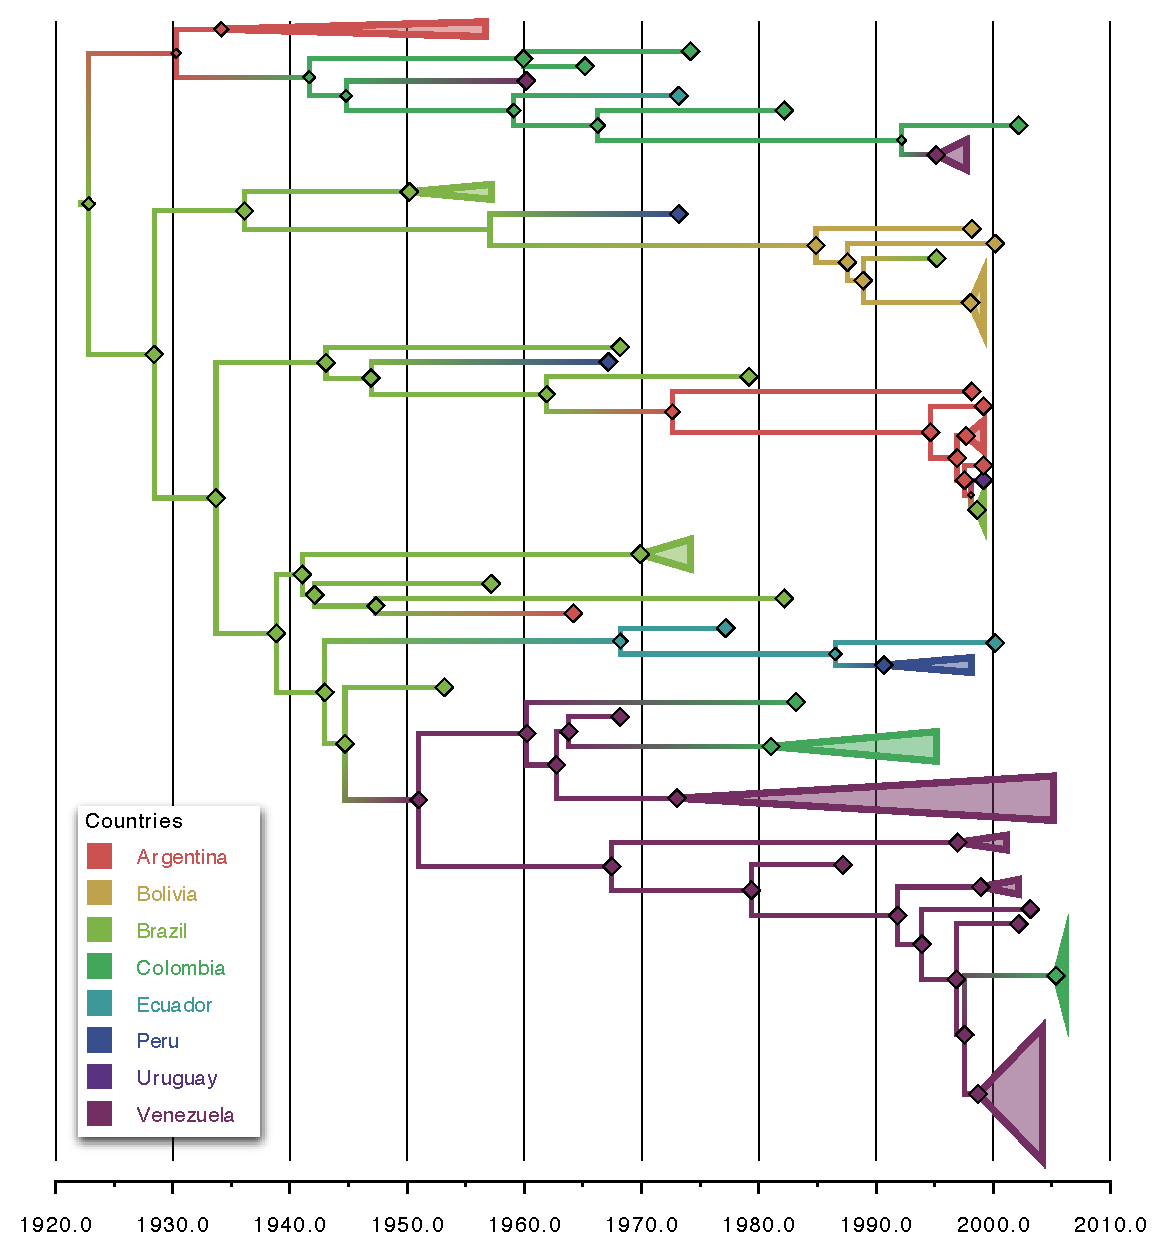
\includegraphics[scale=.45]{FIGURES/A.pdf}}\\
\subfigure[O]{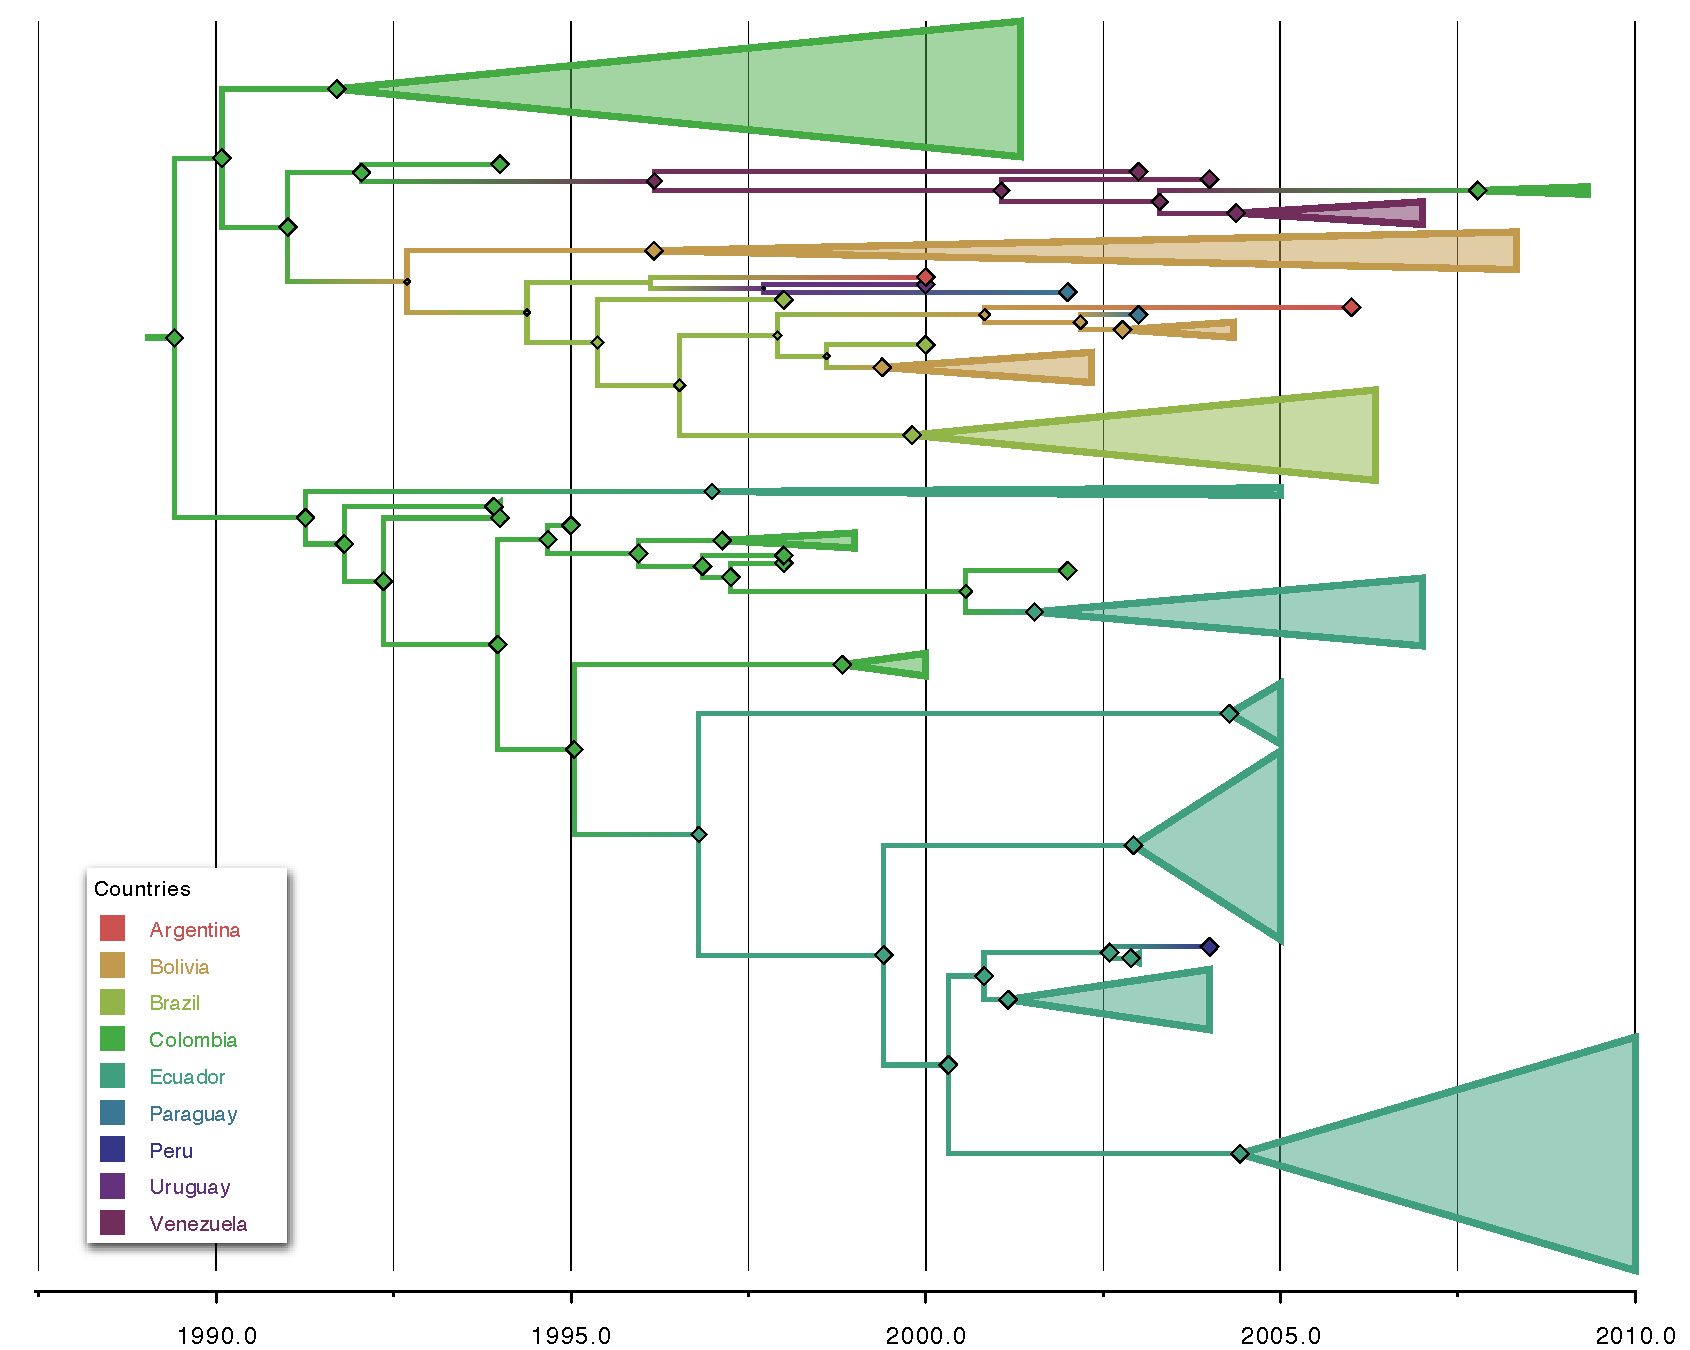
\includegraphics[scale=.30]{FIGURES/O.pdf}}
\end{center}
\caption{}
\label{fig:trees}
\end{figure}
%%%%%%%%%%%%%%%%%%%%%%%%%%
%%%%%%%%%%%%%%%%%%%%%%%%%%
\newpage
\begin{figure}[H]
\begin{center}
\subfigure[A --1945 ]{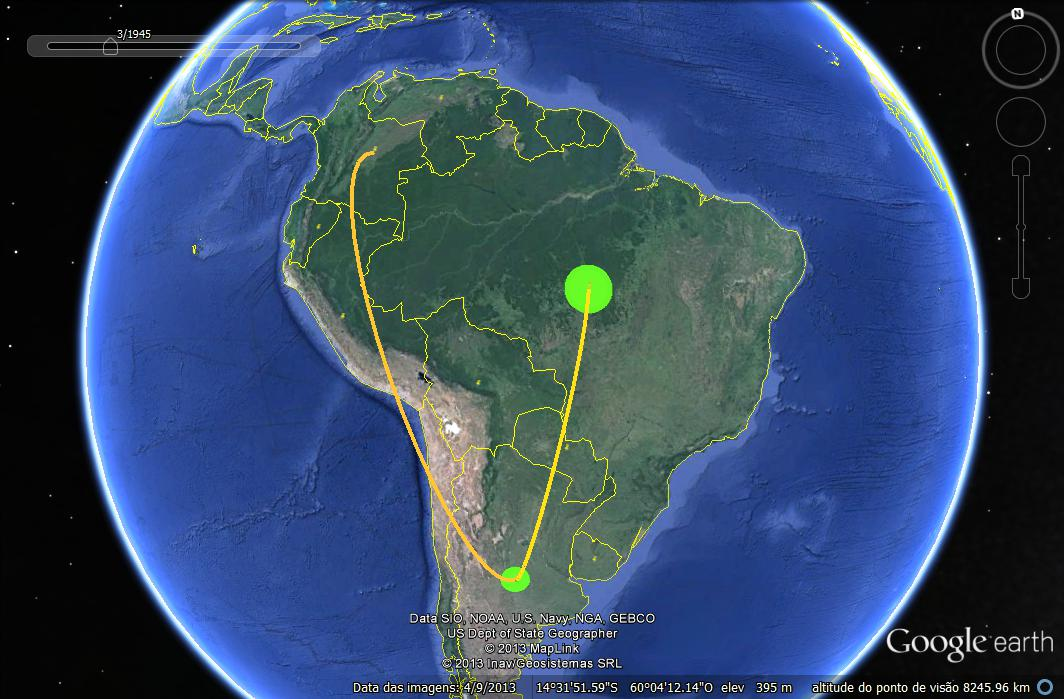
\includegraphics[scale=.20]{FIGURES/A_1945.jpg}}
\subfigure[O --1995 ]{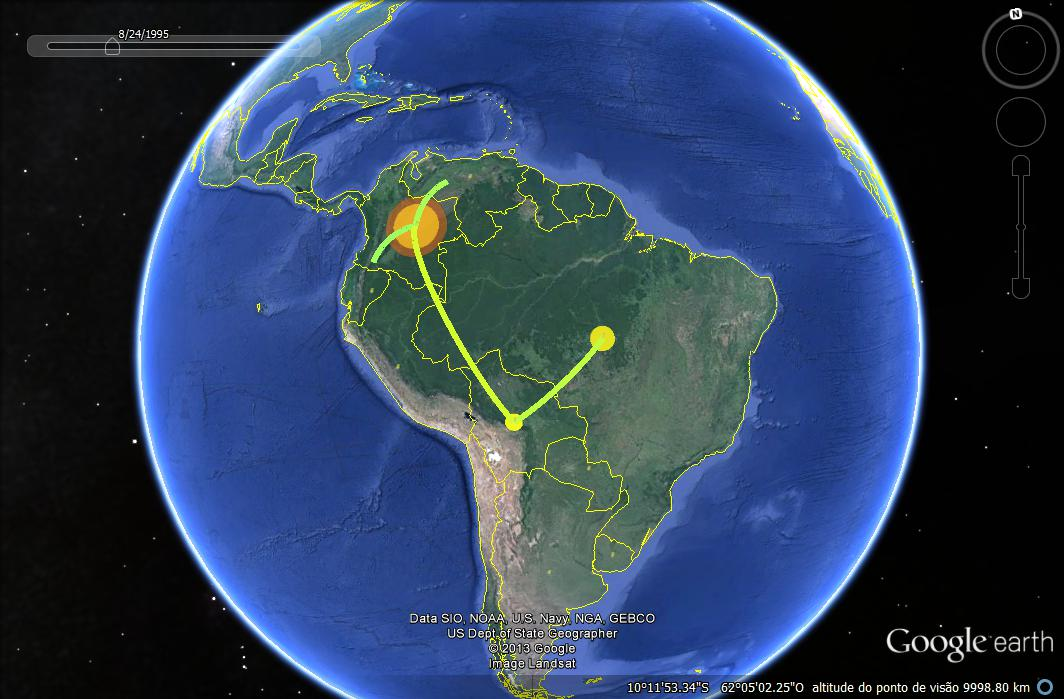
\includegraphics[scale=.20]{FIGURES/O_1995.jpg}}\\
\subfigure[A --1965 ]{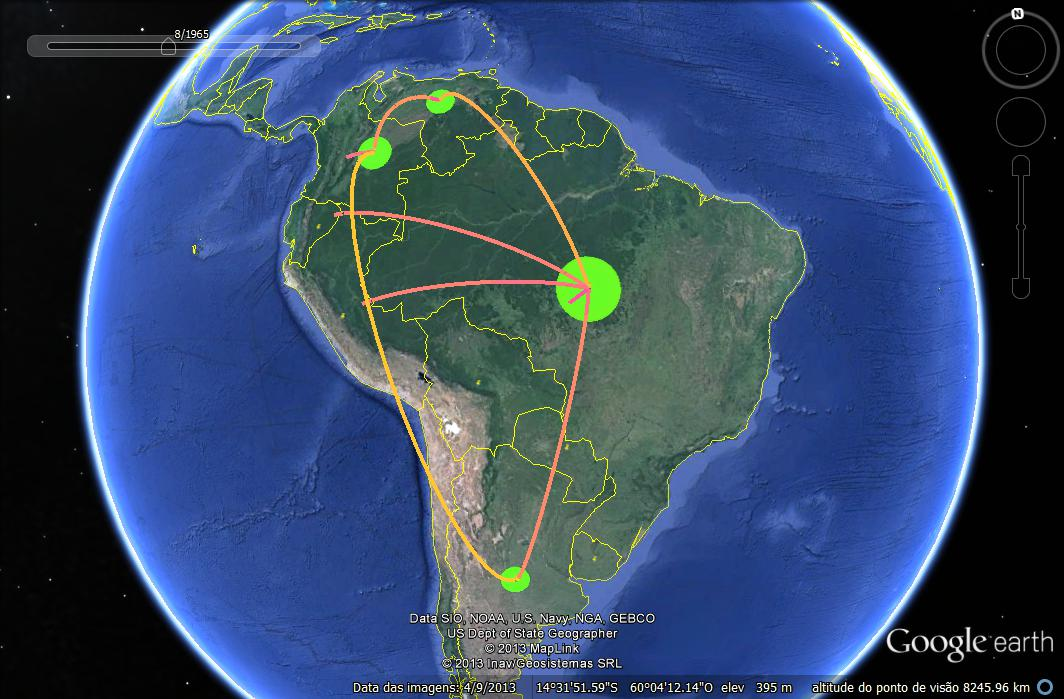
\includegraphics[scale=.20]{FIGURES/A_1965.jpg}}
\subfigure[O --2000 ]{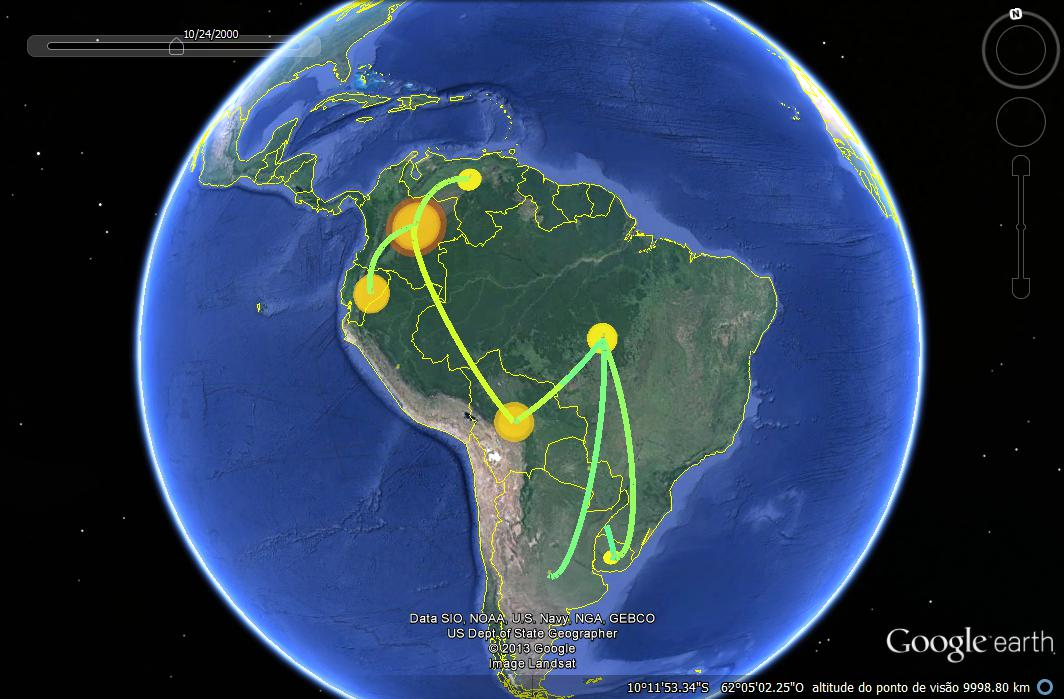
\includegraphics[scale=.20]{FIGURES/O_2000.jpg}}\\
\subfigure[A --1980 ]{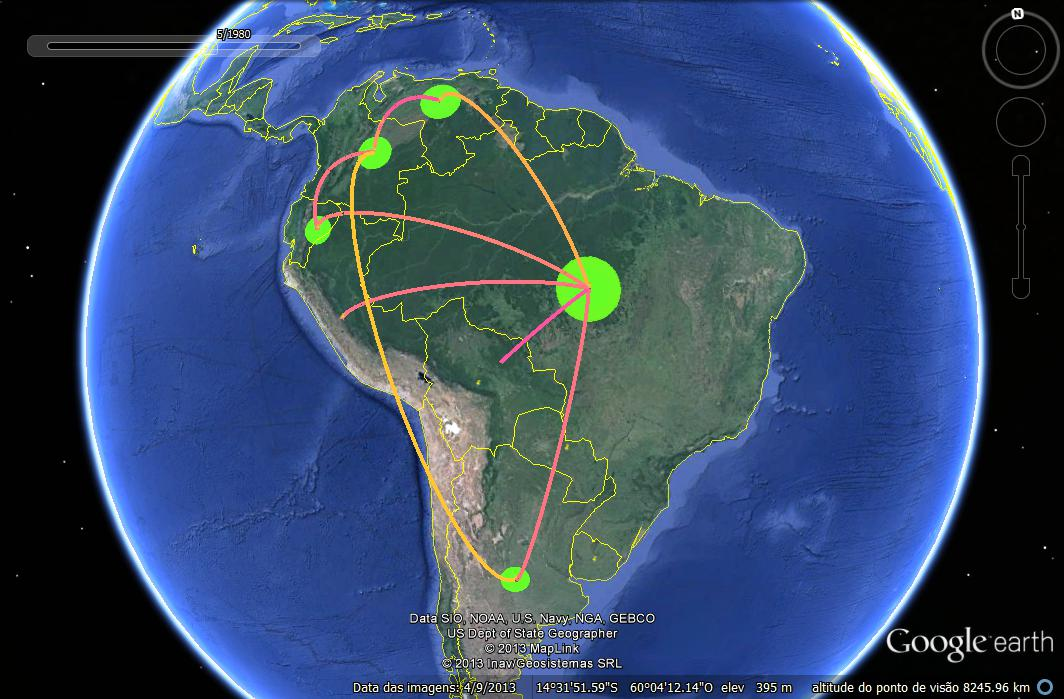
\includegraphics[scale=.20]{FIGURES/A_1980.jpg}}
\subfigure[O --2005 ]{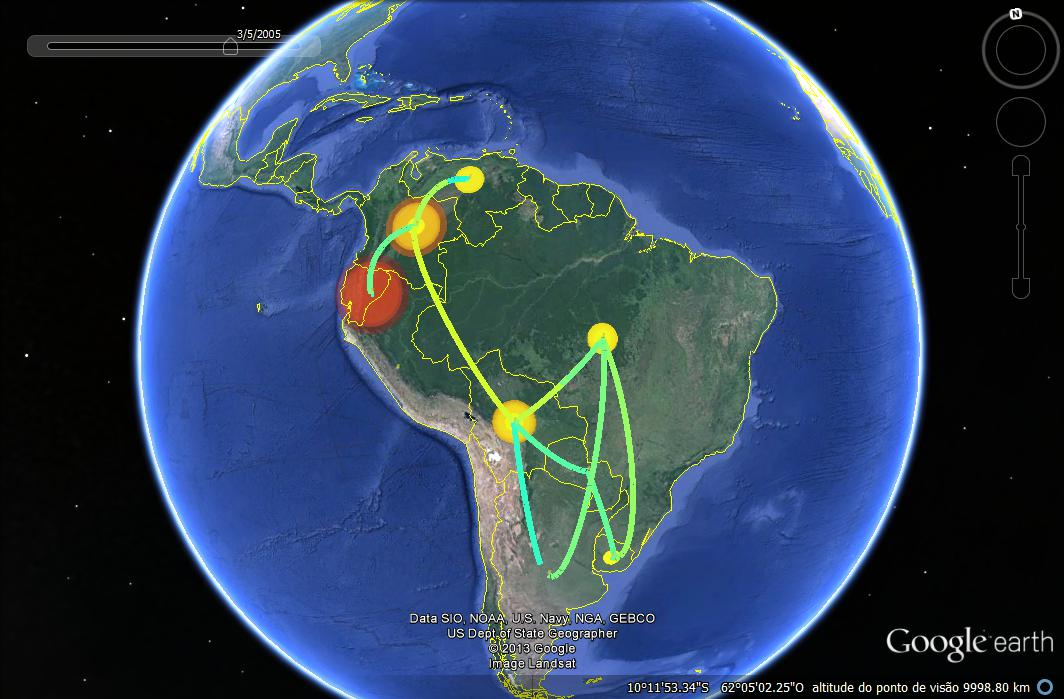
\includegraphics[scale=.20]{FIGURES/O_2005.jpg}}\\
\subfigure[A --2008 ]{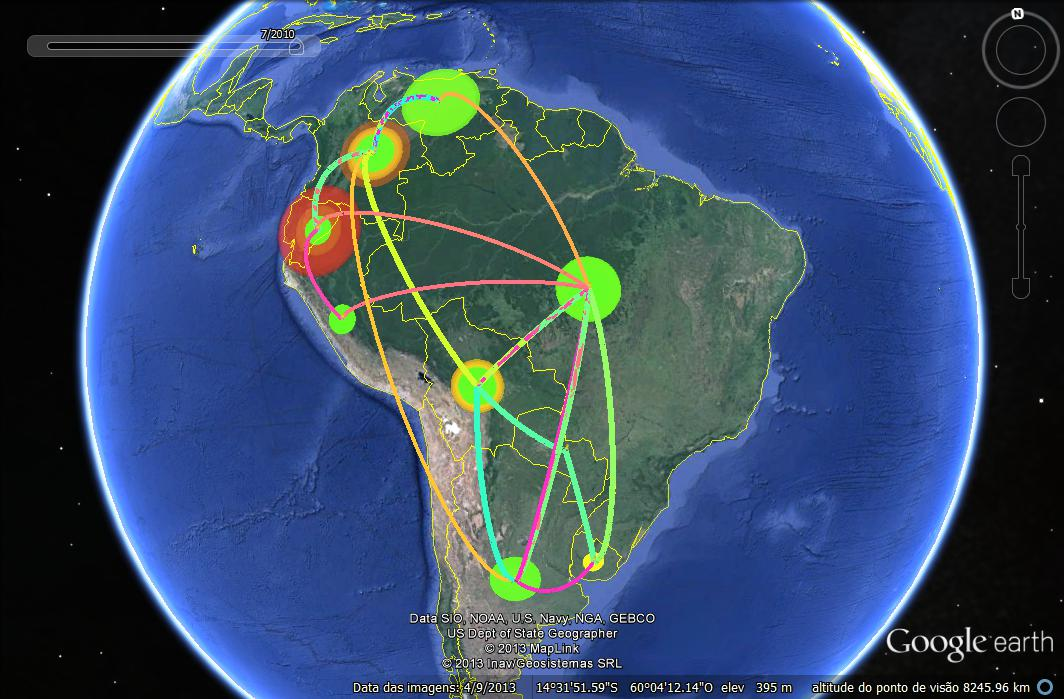
\includegraphics[scale=.20]{FIGURES/A_2008.jpg}}
\subfigure[O --2010 ]{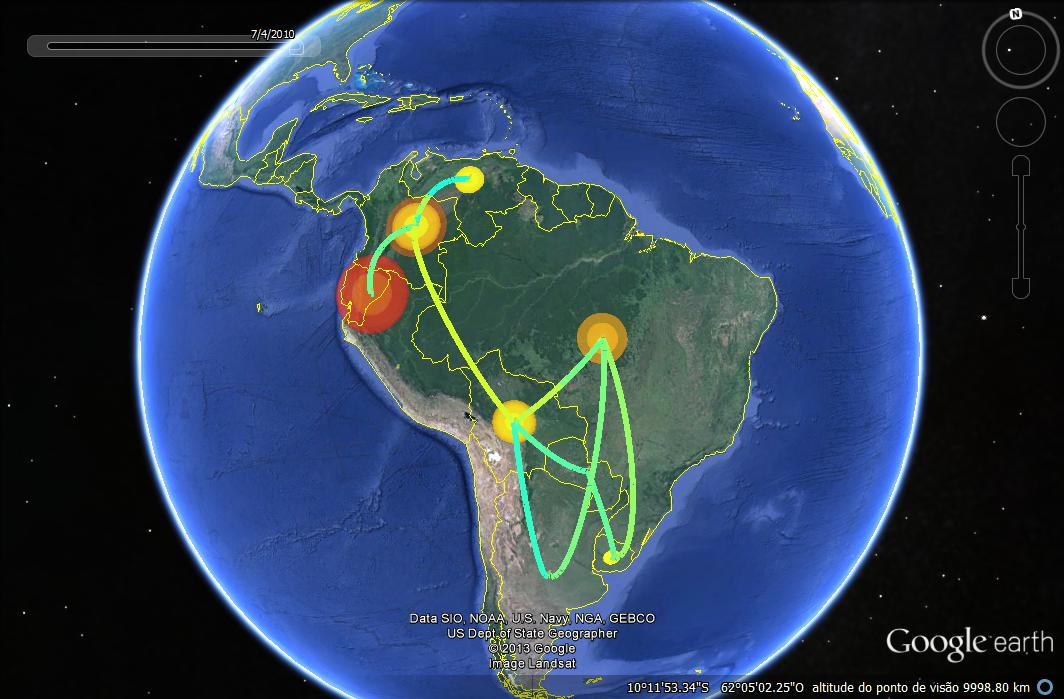
\includegraphics[scale=.20]{FIGURES/O_2010.jpg}}
\end{center}
\caption{}
\label{fig:migration}
\end{figure}
%%%%%%%%%%%%%%%%%%%%%%%%%%
%%%%%%%%%%%%%%%%%%%%%%%%%%
\newpage
\begin{figure}[H]
\begin{center}
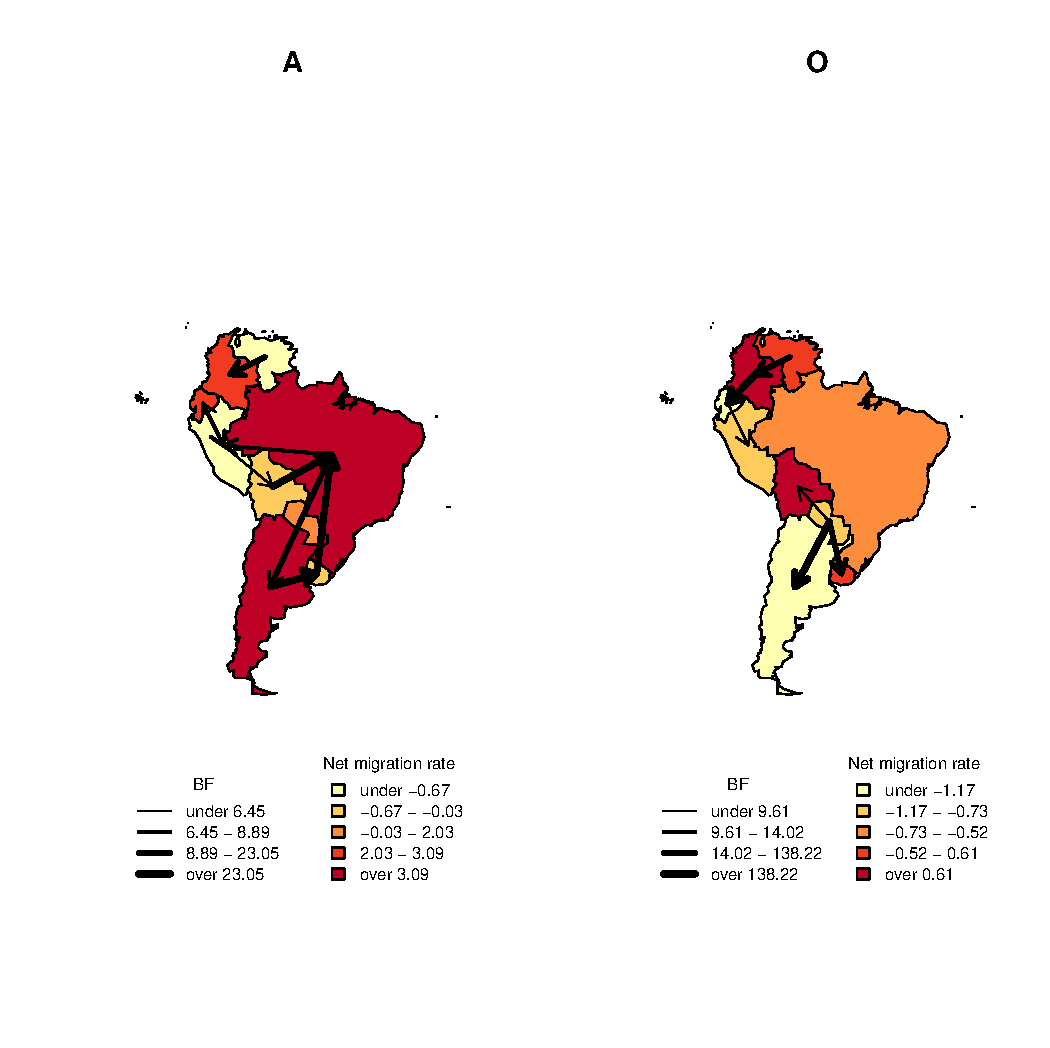
\includegraphics[scale=.85]{FIGURES/compound.pdf}
\end{center}
\caption{}
\label{fig:mj&BFs}
\end{figure}
%%%%%%%%%%%%%%%%%%%%%%%%%%
%%%%%%%%%%%%%%%%%%%%%%%%%%
\newpage
\begin{figure}[H]
\begin{center}
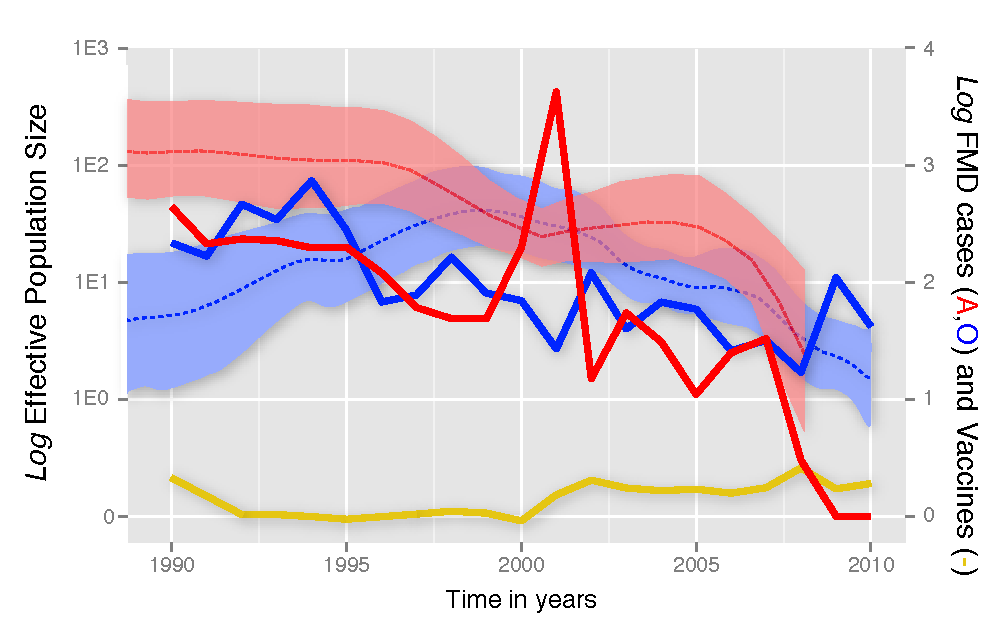
\includegraphics[scale=1.0]{FIGURES/skyride.pdf}
\end{center}
\caption{}
\label{fig:skyride}
\end{figure}
%%%%%%%%%%%%%%%%%%%%%%%%%%
%%%%%%%%%%%%%%%%%%%%%%%%%%
%%%%%%%%%%%%%%%%%%%%%%%% overwritten with each new Beta distribution
\newpage
\begin{table}[H]
\caption{
\textbf{Spatial model selection results for epidemiological predictors.}
We assessed the significance of livestock trade in FMDV spread in South America using two importance sampling methods,  path sampling (PS) and stepping-stone sampling (SS), to estimate (log) marginal likelihoods for each predictor using 64 path steps and 2 million iterations per path step, and corresponding Bayes factor (BF) comparisons.
We also present the (log) marginal likelihood estimates for two location priors under which the location rates are estimated, rather than being fixed (as for the livestock predictors).
%We put these two scenarios in a separate part of the table to indicate that these estimates should not be compared to those of the livestock predictors.
}
\begin{center}
\begin{tabular}{lrrrrrr}
\toprule
 & \multicolumn{3}{c}{Serotype A}& \multicolumn{3}{c}{Serotype O}\\
 \midrule
Predictor & PS & SS & log BF$^2$ & PS & SS & log BF \\
%\hline
Cattle&-12588.76&-12591.26&-27.70&\textbf{-8308.94}&\textbf{-8311.21}& \textbf{13.49}\\
Distance&\textbf{-12557.69}&\textbf{-12559.73}&\textbf{3.83}&-8313.89&-8315.37&9.33\\
Pigs&-12589.33&-12590.94&-27.38&-8325.39&-8326.63&-1.93\\
Sheep&-12570.67&-12572.56&-9.00&-8326.23&-8330.64&-5.94\\
Uniform&-12561.98&-12563.56&--&-8321.49&-8324.70&--\\
\bottomrule
\end{tabular}
\end{center}
\begin{flushleft}
\end{flushleft}
\label{tab:preds}
 \end{table}
%%%%%%%%%%%%%%%%%%%%%%%%
%%%%%%%%%%%%%%%%%%%%%%%%
\newpage
\begin{table}[H]
\caption{
\textbf{Inferred root locations for each predictor for both serotypes.} We present most probable country of origin inferred using each predictor, with associated probabilities inside parentheses. 1-- Uniform, all rates equal prior; 2-- Probability of being the root; 3-- Kullback-Leibler Divergence.
}
\begin{center}
\begin{tabular}{lcccc}
\toprule
& \multicolumn{2}{c}{Serotype A}&\multicolumn{2}{c}{Serotype O}\\
Predictor& Origin ($Pr$(root)$^2$)& KL$^3$&Origin ($Pr$(root))& KL\\
\midrule
Distance & Argentina (0.75)&3.86& Colombia (0.96)&3.76\\
Sheep    & Brazil (0.89) &3.52 & Colombia (0.99)&5.91\\
Pigs      & Colombia (0.99)& 5.98&Colombia (0.91)&4.73\\
Uniform$^1$  & Argentina (0.84)& 3.78&Colombia (0.96)&3.20\\
Cattle   & Peru (0.93)& 5.17 &Colombia (0.95)&3.81\\
 \bottomrule
\end{tabular}
\end{center}
\begin{flushleft}
\end{flushleft}
\label{tab:roots}
 \end{table}
%%%%%%%%%%%%%%%%%%%%%%%%
\end{document}
